\documentclass[a4paper,12pt]{article}

\usepackage{fancyhdr}
\usepackage{lastpage}
\usepackage{amsmath}
\usepackage{tikz}
\usepackage{amsfonts}
\usepackage{csvsimple}
\usepackage{graphicx}
\pagestyle{fancy}

\linespread{1.6}

\lhead{Samuel Loomis}
\setlength{\headheight}{15pt}
\chead{Thesis Methods}
\rhead{\thepage\ of \pageref{LastPage}}
\lfoot{}
\cfoot{}
\rfoot{}

\begin{document}
\section*{Methods}

Monte Carlo simulations are used to generate average sphere locations over many thousands of itterations.    Monte Carlo simulations take a randomized configuration of spheres and attempt to make a small move for each sphere. 
\begin{figure}[h]
\centering
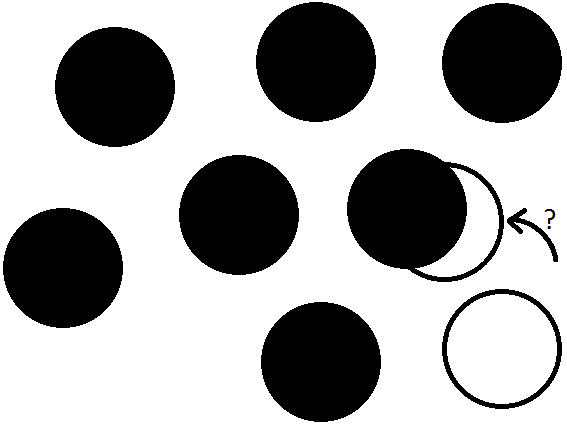
\includegraphics[width=1.5in]{Sample_Move.PNG}
\caption{Example of a move}
\end{figure}\\
 When a sphere moves it interacts with other spheres and the total energy of the system changes.  The move is accepted if it passes a Boltzmann factor probability check:  $P=e^{-\beta\Delta E}$.  If the energy after a move is completed is lower than before, the move is always accepted because the Boltzmann factor check will always be greater than 1.  If the energy is higher, the move may or may not be accepted, as the change in energy goes up, the chance of a successful move goes down.  One itteration is complete after every sphere has had a chance to move.  After every itteration, the location of each sphere is saved, and the final output is the average location of the spheres over all the itterations completed.  The simulations are allowed to run for extended periods of time on the OSU quipu cluster.  The plot shown on the next page is from a simulation that has 36 million iterations completed and is still under 1\% "complete".

To observe different characteristics of fluids, the Monte Carlo simulation can be ran under different configurations.  The two configurations primarliy observed are the Homogeneous and Wallz.
The wallz configuration is used to observe how the spheres settle near a wall constraining the spheres in the z direction.
\begin{figure}[h]
\centering
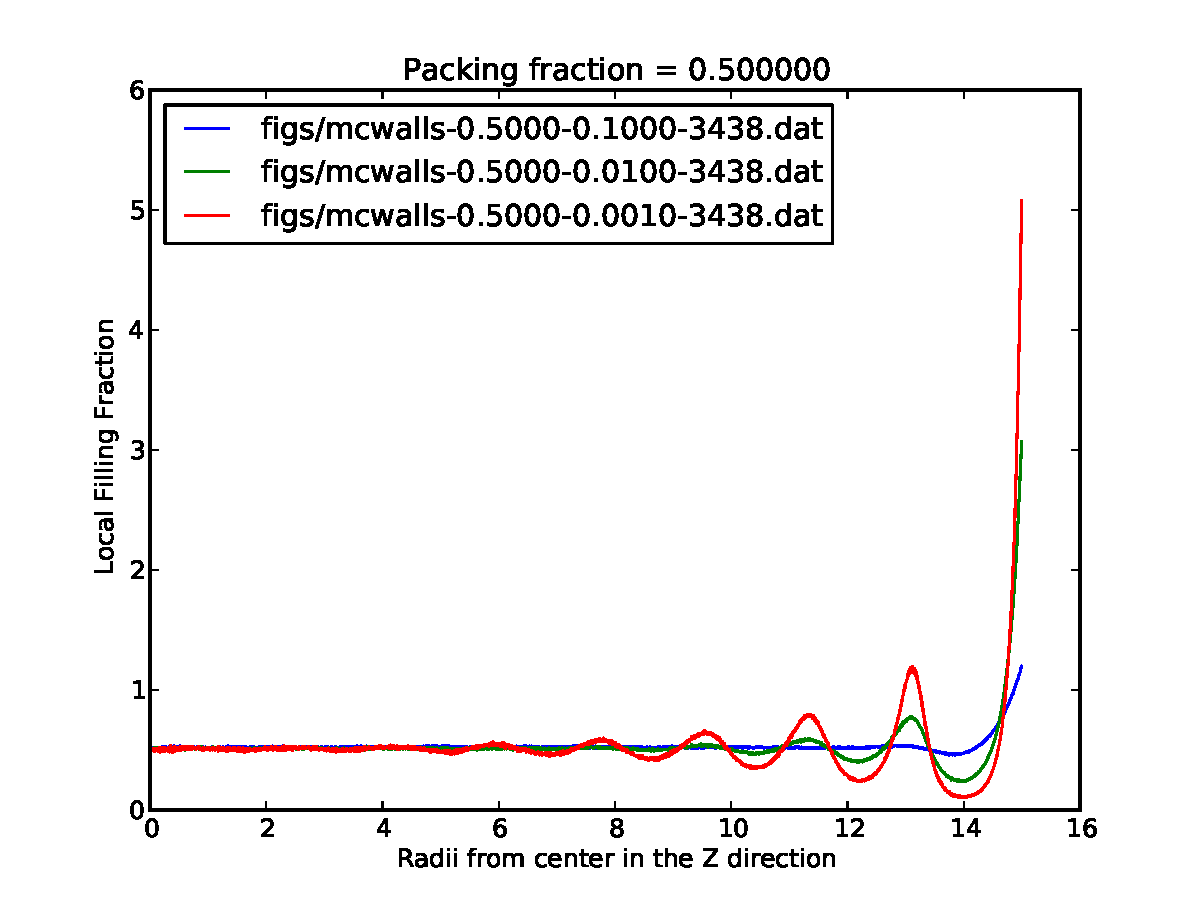
\includegraphics[width=3in]{walls-50.pdf}
\caption{Monte Carlo Wall Z Density plot after 36 million itterations.}
\end{figure}\\
The Homogeneous simulation is used to obtain radial distribution functions.  These functions, knowing that 1 sphere is located at the origin, show the probablility that another sphere will be found a certain distance away.
\begin{figure}[h]
\centering
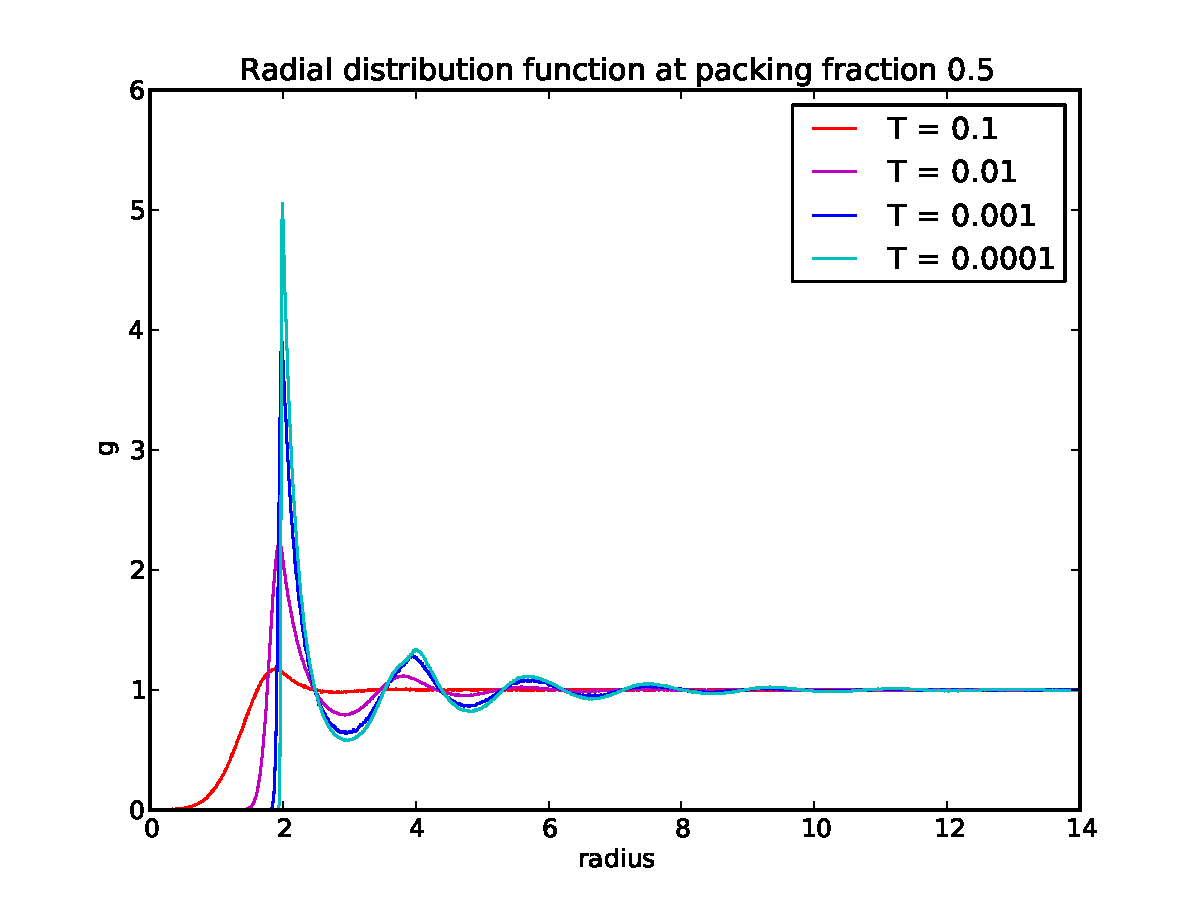
\includegraphics[width=3in]{radial-distribution-50.pdf}
\caption{Example of Radial Distribution Functions}
\end{figure}\\



\end{document}
